% begin module limits-ex7
\begin{frame}
By comparing definitions, we can see that
\[
\lim_{x\rightarrow a} f(x) = L \ \text{ if and only if } \lim_{x\rightarrow a^-}f(x) = L \ \text{ and } \lim_{x\rightarrow a^+}f(x) = L .
\]
\begin{example} %[Example 7, p. 100]
\begin{columns}[c]
\column{.55\textwidth}
The graph of a function $g$ is shown to the right.  Use it to state the values (if they exist) of the following:



\[\begin{array}{r@{~}c@{~}l|r@{~}c@{~}l}
\displaystyle \alertNoH{ 2-3}{\lim_{x\rightarrow 1^-}g(x)} & \alertNoH{2-3}{=}& \fcAnswer{3}{3} &%
\displaystyle \alertNoH{ 8-9}{\lim_{x\rightarrow 3^-}g(x)} & \alertNoH{8-9}{=}& \fcAnswer{9}{1} \\%
\displaystyle \alertNoH{ 4-5}{\lim_{x\rightarrow 1^+}g(x)} & \alertNoH{4-5}{=}& \fcAnswer{5}{3} &%
\displaystyle \alertNoH{ 10-11}{\lim_{x\rightarrow 3^+}g(x)} & \alertNoH{10-11}{=}& \fcAnswer{11}{2} \\%
\displaystyle \alertNoH{ 6-7}{\lim_{x\rightarrow 1}g(x)} & \alertNoH{6-7}{=}& \fcAnswer{7}{3} &%
\displaystyle \alertNoH{ 12-13}{\lim_{x\rightarrow 3}g(x)} & \alertNoH{12-13}{=}& %
\displaystyle  \fcAnswer{ 13}{\text{DNE}} %
\end{array}
\]
\column{.45\textwidth}
\psset{xunit=0.9cm, yunit=0.9cm}
\begin{pspicture}(-0.5, -0.5)(5.3,5.1)
\psframe*[linecolor=white](-0.5,-0.5)(5.3,5.1)
\tiny
\psaxes{<->}(0,0)(-0.5,-0.5)(5.2,5)
\fcLabels{5.2}{5}
%Function formula: 37/10+9/20 (x)+7/20 ((x)^{3})-3/2 ((x)^{2})
\psplot[linecolor=red, plotpoints=1000]{-0.5}{3}{x 2 exp -1.5 mul x 3 exp 0.35 mul x 0.45 mul 3.7 add add add }
%Function formula: 3/2+1/2 ((-4+x)^{2})
\psplot[linecolor=red, plotpoints=1000]{3}{5}{x -4 add 2 exp 0.5 mul 1.5 add }
\rput[lb](1.6,2.3){$y=g(x)$}
\fcFullDot{1}{4}
\fcHollowDot{1}{3}
\fcHollowDot{3}{1}
\fcHollowDot{3}{2}
\end{pspicture}
% 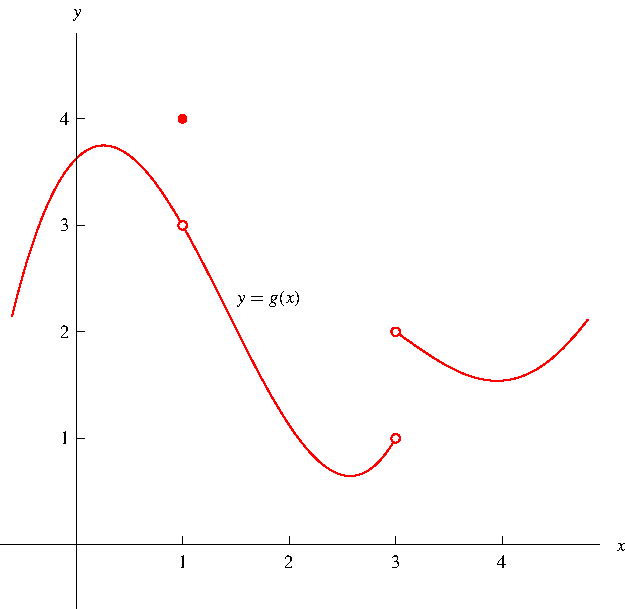
\includegraphics[height=5cm]{limits/pictures/02-02-ex7.pdf}%
\end{columns}
\end{example}
\end{frame}
% end module limits-ex7
